  \documentclass[a4paper, 11pt]{article}
\usepackage[utf8]{inputenc} 
\usepackage[T1]{fontenc}
\usepackage{graphicx}
\usepackage[french]{babel} 
\usepackage{multirow,multicol}
\usepackage{amsmath, amssymb, latexsym}
\usepackage{pstricks,pst-node,pst-coil,pst-grad,pst-plot}
\usepackage{epsfig,subfigure}
\usepackage[lined,boxed]{algorithm}
\usepackage{algorithmic}
\usepackage{rotate}
\usepackage{url}
\usepackage{hyperref}
\usepackage{setspace}

\newtheorem{definition}{Definition}
\newtheorem{example}{Example}
\newtheorem{proposition}{Proposition}
\newtheorem{proof}{Proof}

\title{Présentation d'un Manic'shooter}
\author{Nicolas.Aubry - David.Ragot - Théo.Berthier} 


\begin{document}

\maketitle
\tableofcontents
\section{Manic Shooter}
\subsection{Présentation-Objectif}

Présentation d'un Manic Shooter:
Manic shooter ou Shoot them up ou Shmup qui signifie littéralement "Descendez-les tous".
Un Manic shooter est un jeu ou le joueur doit diriger un personnage ou un véhicule devant tuer un grand nombre d'ennemis à l'aide d'armes de plus en plus puissantes au fur et à mesure des niveaux, le personnage doit esquiver les tirs ou les projectiles venant des ennemis.
Ce système de jeu est sorti en 1978 avec 
\href{http://dictionnaire.sensagent.leparisien.fr/Space%20Invaders/fr-fr/}{Space inverders}
 present dans les salles d'arcades de base c'est un jeu 2D il trouve son succès vers la fin des années 80. Début des années 90 dès que le graphisme tri-dimensionnelle sont apparut, son succès disparut au profit des jeux 3D.

 \begin{figure*}[ht!]
 \centering
 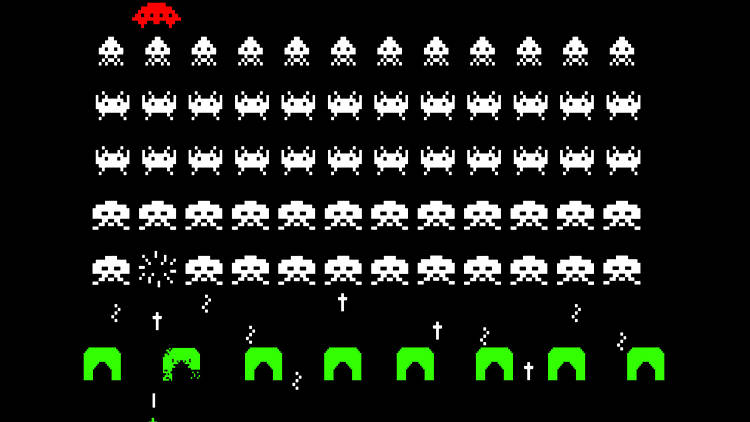
\includegraphics[width=0.7\linewidth]{space.jpg}
 \caption{Space inverders}
 \label{fig::example::one}
\end{figure*}

\section{Architecture}


 \begin{figure*}[ht!]
 \centering
 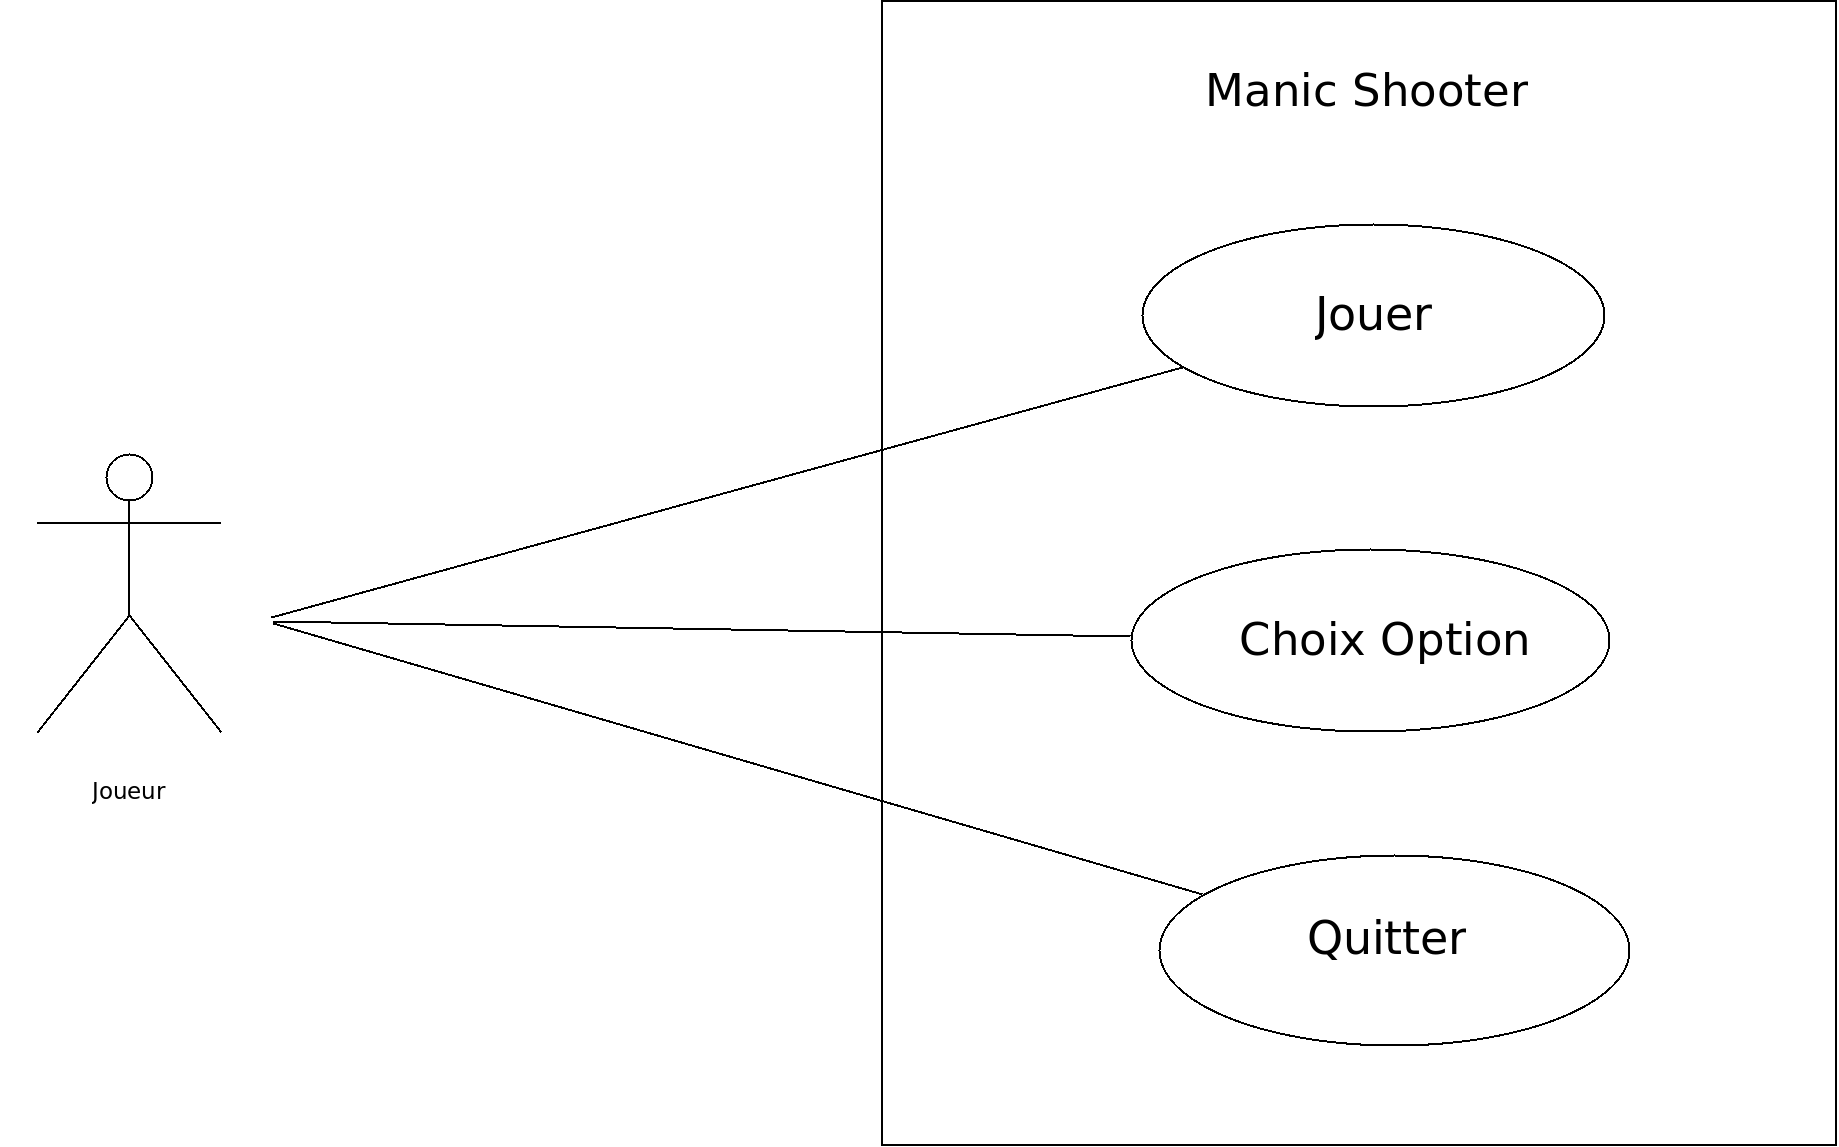
\includegraphics[width=1.1\linewidth]{diagfinal.png}
 \caption{diagramme cas d'utilisations}
 \label{fig::example::one}
\end{figure*}

Ici nous avons à faire dans le premier menu. Il propose deux bouttons différents. Un qui va proposer de jouer , un autre de Quitter. Et enfin une liste de résolution prédéfinies. Pour pouvoir choisir une résolution adaptée aux différents ordinateurs.
Jouer lance pygame et donne accès au menu final du jeu ou lancer le jeu est possible ou de changer des paramètres comme les préférences de jeu du joueur.


\section{Fonctionnalité du jeu}


 	\subsection{Une carte}
 	
 	\begin{figure*}[ht!]
\centering
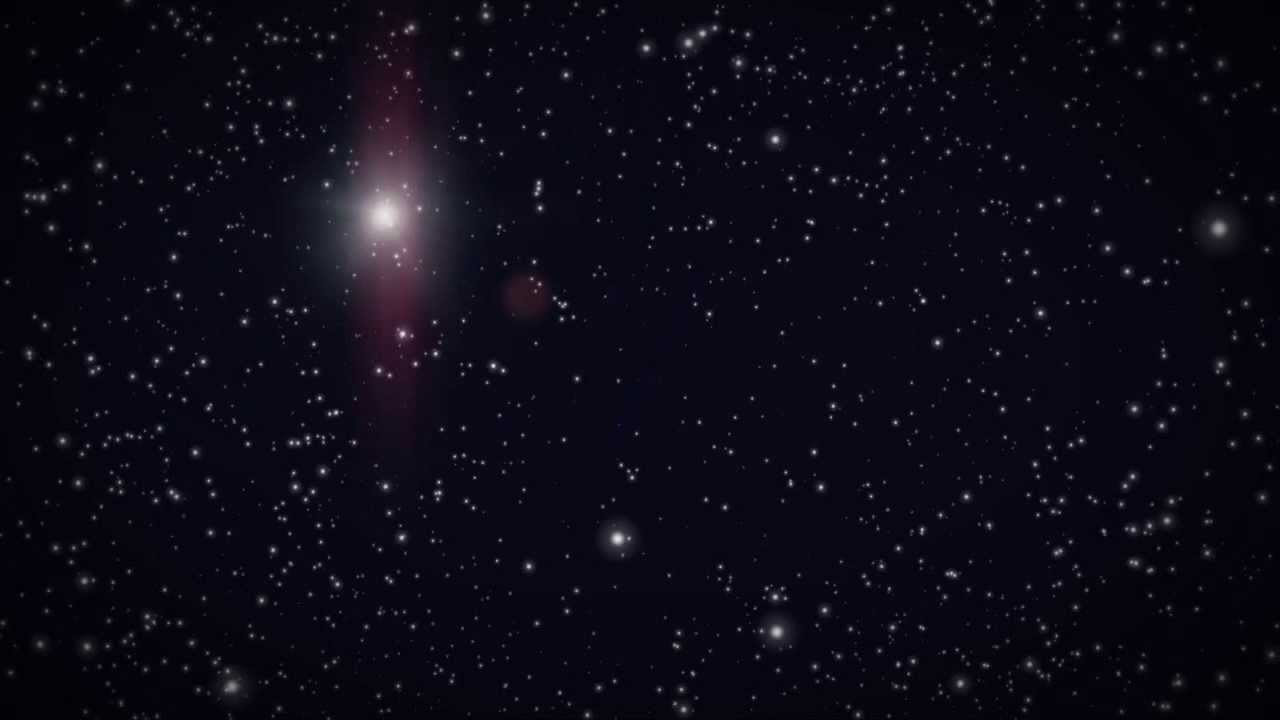
\includegraphics[width=0.8\linewidth]{Background.jpg}
\caption{Notre carte}
\end{figure*}
 	dans un premier temps il nous fallait une carte, c'est à dire un espace de jeu permettant à un héro d'évoluer dans un espace rempli d'ennemis et d'être livré à une épopée, une histoire. 
 	notre premier réflexe a était de créer une grille et de créer un héro en l'initialisant avce le caractère "1", et en initialisant des ennemies avec le caractère  "0". Le reste de la grille étant que des caractères  "-", représentant le vide. Menant notre objectif jusqu'au bout nous nous sommes rendu compte qu'en associant l'interface graphique avec notre modèle de jeu. Cela posait problème et surtout qu'il existait une manière "plus simple" de faire la carte et de manière plus efficace. Car en définissant la fenêtre avec Pygame cela aller être notre grille, donc notre espace de jeu. C'est à dire que la grille est égale à la taille de fenêtre fois le nombre de pixels. Ce qui nous à simplifié la vie pour la suite, car la gestion avec la fenêtre est intégré à Pygame.

 	
	\subsection{Un personnage}
Un manic shooter a pour habitude d'avoir un héro qui se déplace dans la carte, dans l'espace que l'on aurat défini. Il nous fallait donc un héro ou personnage qui soit celui que le joueur puisse contrôler notre personnage :
\begin{figure*}[ht!]
\centering
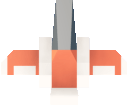
\includegraphics[width=0.1\linewidth]{spaceCraft1.png}
\caption{Notre personnage trouve sur internet "open source"}
\end{figure*}
Ce personnage est équipé d'un réacteur qui le suit, il a fallu intégrer cela au déplacement du héro, et de faire en sorte que le réacteur soit collé au calque du personnage, donc de son vaisseau. Il a fallu donc que la position soit identique pour le réacteur est pour le vaisseau du personnage .... suite .....

	\subsection{Des ennemis}
Le héro n'est pas le seul personnage à gérer. Il nous faut également gérer les ennemies. En ce qui concerne les ennemies nous avons choisit de gérer le pseudo-aléatoirement; C'est à dire que l'on a utilisé une fonction qui permet de générer les ennemies en fonction de la vague dans laquelle on se trouve. Et de ne pas avoir trop d'ennemis dès le début de partir. Mais que le manière d'apparaître soit de plus en plus importante. Mais reste toujours accessible pour le joueur. Les ennemis apparaissent dans un coin en haut de l'écran, non visible pour le joueur. Et après ils suivent la trajectoire, le déplacement qui leurs sera attribués.

	\subsection{Déplacement}
Une fois le contexte posé pour les personnages / la carte, c'est maintenant qu'intervient la notion de déplacement évidement le héro doit se déplacer pour éviter les ennemies et avant dans sont épopée, mais les ennemies doivent se déplacer également, il se déplace aléatoirement pour atteindre le héro pour cela nous allons utiliser la librairie random qui génère des chiffres aléatoire ce qui nous permet d'associer cela à aux déplacements.
Au début les déplacements étaient de la "téléportation" c'est à dire que la position du héro était traité avec des rafraîchissement d'images c'est à dire, quand le joueur appuie sur la touche déplacer le héro change de position et donc une nouvelle image et crée sur cette position. L'ancienne image est donc supprimé. Mais cela pose un problème, quand la vitesse du héro est trop grande on voit les différentes images des différentes positions du héro, ....... suite .......
	
	\subsection{Tir}
Généralement dans un manic shooter le héro doit posséder un tir qui va détruire les ennemies 
	\subsection{collisions}
Les personnages sont confronté à des collisions qui doivent être gérées, c'est à dire quand le tir va allé toucher un ennemi, ou le vaisseau du joueur. Le tir est prévu pour avec des points de dégâts, qui peuvent être changés dans le SHOP que l'on a mis en place. Cela permet au joueur d'acheter des tirs avec plus ou moins de dégâts, ainsi que des tirs de natures différentes. Le joueur pourra si il le souhaite, avoir des doubles, quadruple tirs. Ou encore des tirs entrelacés. 

\section{Éléments techniques}

\subsection{Python}

Pour ce projet nous utilisons python 3 avec 10 librairie externe à python :
OS,sys,pygame,tkinter,random,json,time,sympy

\subsection{Choix de l'interface graphique}

Le choix des utilitaires utilisés peut différer le rendu du projet. Nous avons donc dû tester au fur et à mesure ce qui aller nous convenir le mieux, et permette d'avoir une expérience utilisateur qui nous paraissait la meilleure possible de notre point de vu.

\subsection{Tkinter}
tkinter est une interface graphique qui est orientée logiciel elle permet la création de menu beaucoup plus simple dans notre cas cela nous sert pour le premier menu de notre jeu. En effet la création de boutons y est assez simple ainsi que leurs positionnement au sein de la fenêtre. du faite que les boutons sont directement implémentés dans la librairie de tkinter.
 \begin{figure*}[ht!]
 \centering
 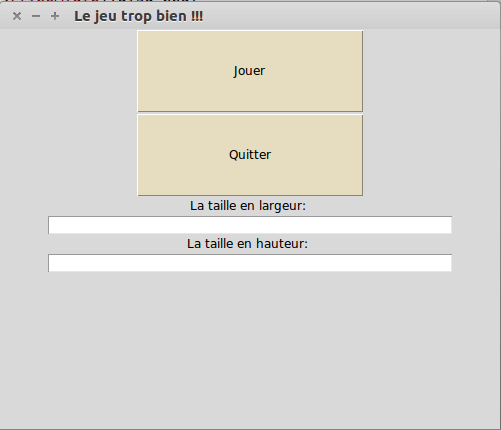
\includegraphics[width=0.7\linewidth]{tkinter.png}
 \caption{Notre premier menu avec tkinter}
 \label{fig::example::one}
\end{figure*}

\href{https://www.tutorialspoint.com/python/python_gui_programming.htm}{source tkinter}

\subsection{Pygame}
Pygame est également une interface graphique qui est plus destinée au jeu.
Dans notre cas nous l'utilisons pour l'intégralité de notre gameplay , les déplacement, les collisions , la carte, les tirs ainsi que pour plein d'autre choses. Le choix de cette interface graphique nous est venu naturellement car elle offre des possibilités de déplacements intéressante, ainsi que la création de toute les animations liées au jeu. Pygame est très interressant pour cela. Le seul bémole que nous pouvons lui reprocher, est son manque de documentation sur le site officiel. Ce qui rend la compréhension des fonctionnalités ainsi que des fonctions propres à Pygame assez difficile.
 \begin{figure*}[ht!]
 \centering
 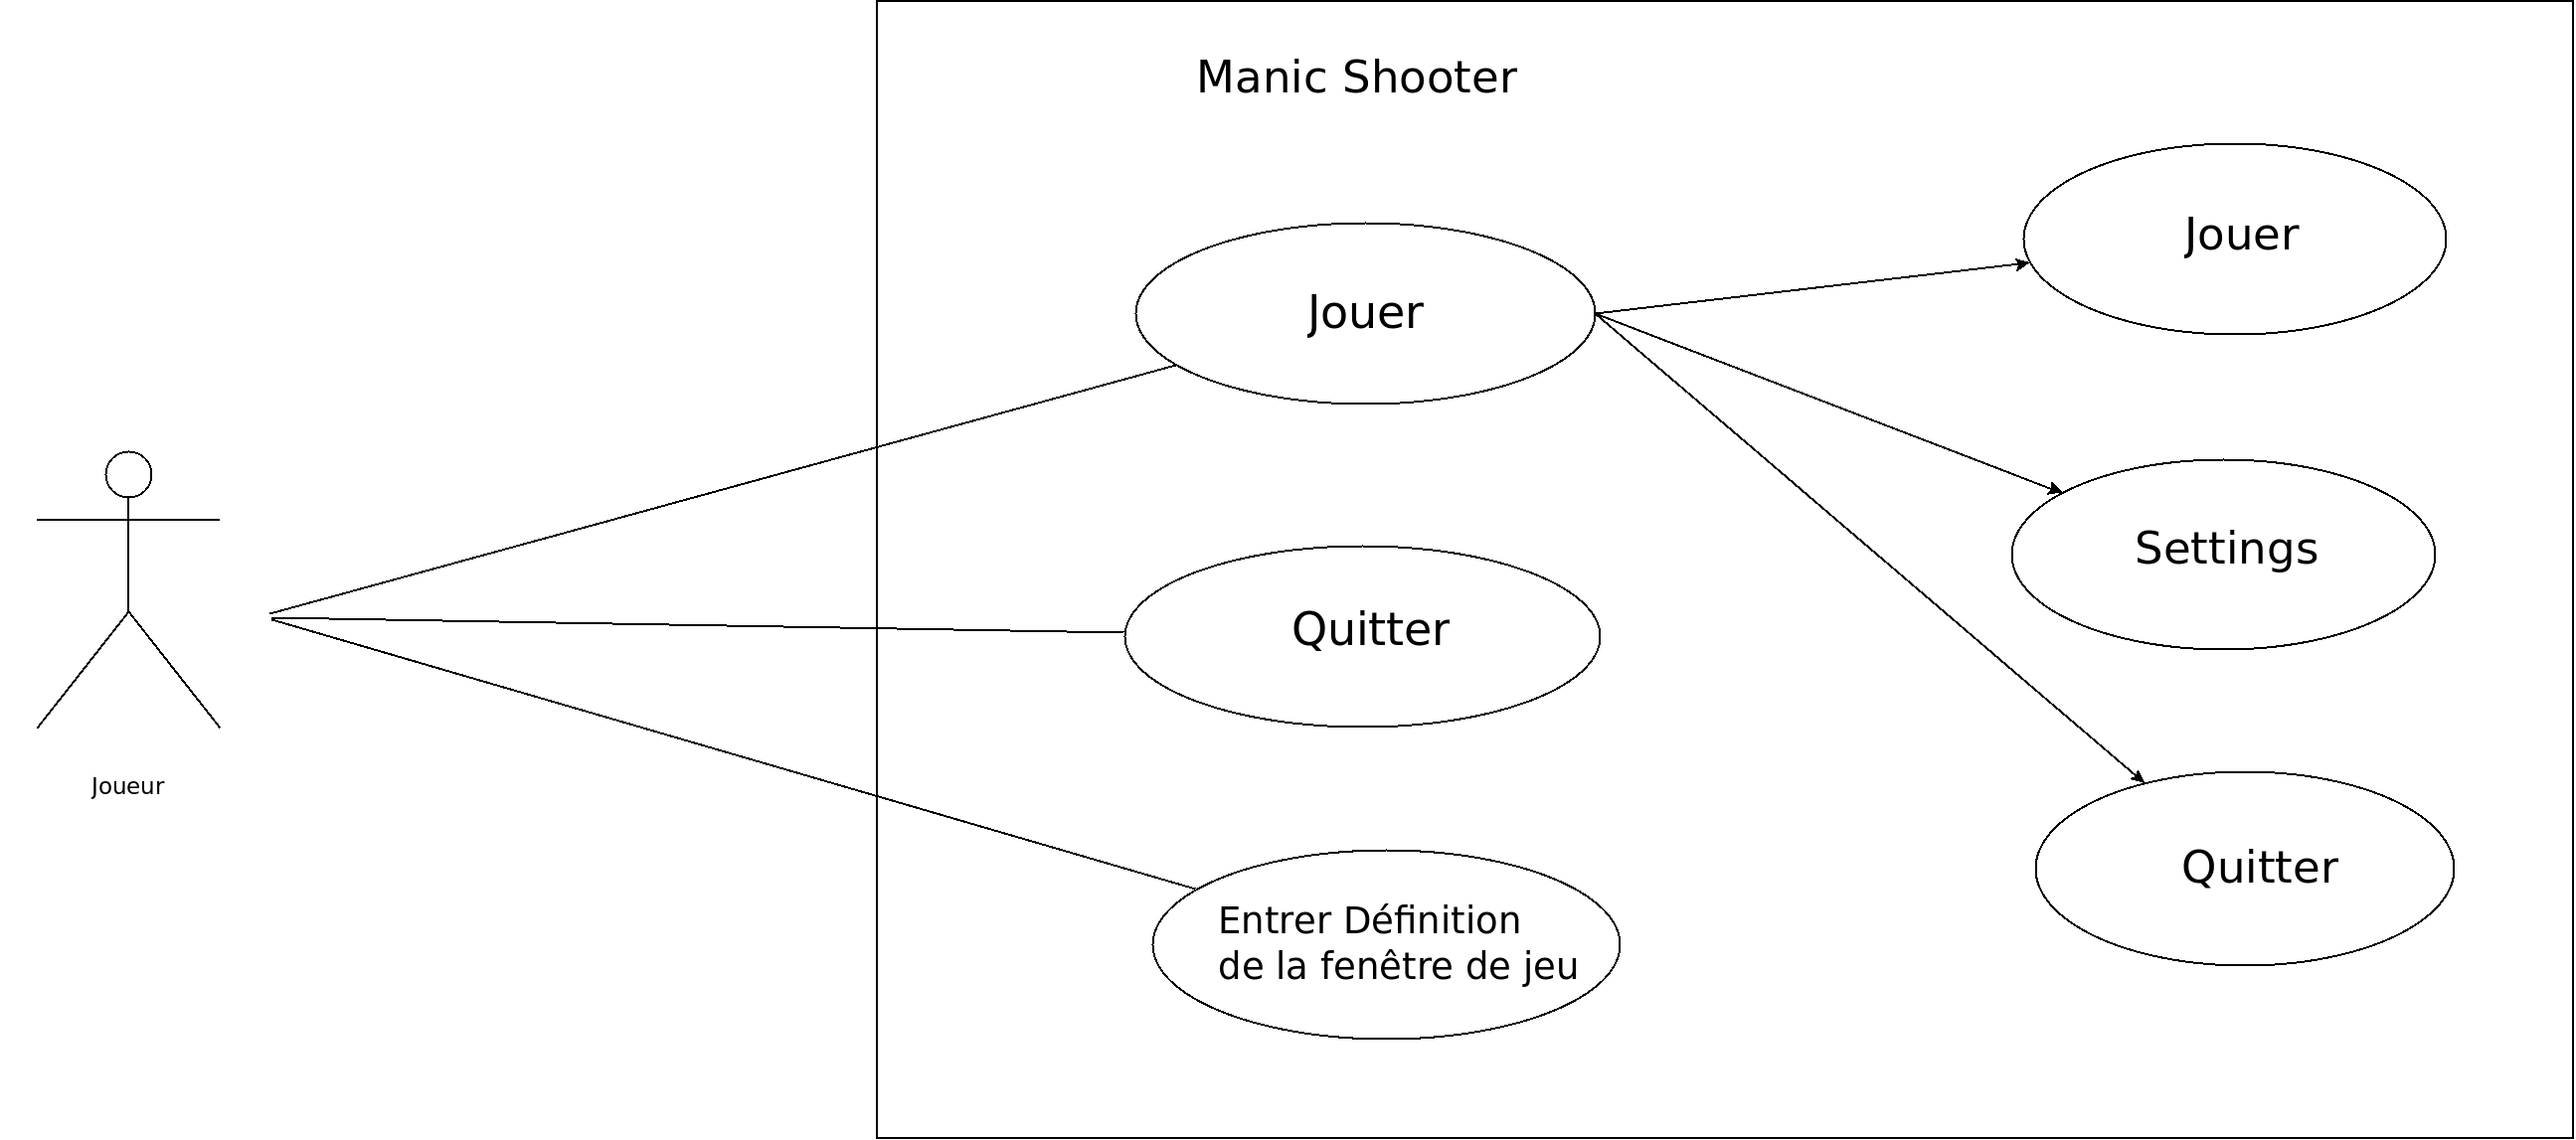
\includegraphics[width=0.5\linewidth]{diag.png}
 \caption{Gameplay avec pygame}
 \label{fig::example::one}
\end{figure*}

\href{http://www.pygame.org/docs/}{source pygame}

\section{Expérimentation et Usages}
capture d'écran rendu final / perfomance 

\subsection{Expérimentation}
Une phase d'expérimentation à du être nécessaire pour identifier ce qui peut poser problème.
Pour commencer nous avons penser initialiser une grille pour la carte et des personnages étant des numéros pouvait traverser la grille. Nous nous sommes vite rendu compte que cela aller poser problème cela ne rendait pas le jeu dynamique, et nous étions obligé de faire un déplacement de vaisseau du joueur pour que la grille puisse se mettre à jour.
Une fois que nous avons ouvert la fenêtre de Pygame nous nous somme rendu compte que la grille aller devenir cette fenêtre et que les déplacements vont se faire plus dynamiquement grace à cette manière. Nous avons donc oublié la grille.
Le choix des interface graphique c'est fait en essayant dans un premier temps tkinter. Tkinter a était sollicité et nous nous sommes rendu compte que le rendu graphique n'était pas de qualité, les menus se faisaient facilement donc le premier menu c'est fait avec celui ci. Mais pour la conception du jeu c'est Pygame qui à était retenu, car il était plus fléxible pour la partie gameplay ainsi que pour beaucoup d'autres choses au sein de notre projet.

\subsection{Usages}
Pour l'usage de notre jeu
\section{Conclusion}
\end{document}
